\chapter{ Аналитический раздел}
\label{cha:analysis}
%
% % В начале раздела  можно напомнить его цель
%
Lorem ipsum dolor sit amet, consectetur adipiscing elit. Integer a mauris consequat, sagittis odio ut, tempor lacus. Donec rhoncus tincidunt ligula, vel egestas turpis vehicula interdum. Phasellus sit amet dignissim metus, quis rutrum metus. Nullam euismod dictum rhoncus. Vivamus bibendum gravida lacus, iaculis consectetur nunc suscipit ac. Aliquam erat volutpat. Nulla laoreet, elit vel lacinia egestas, metus erat sagittis orci, quis vulputate urna tellus ut felis. Morbi sit amet elit auctor, ultrices dui eu, elementum nisi.

Proin at ipsum non nulla rutrum iaculis at eget sapien. Morbi rhoncus urna sed vulputate vulputate. Etiam gravida diam a sem egestas, eget tincidunt purus lobortis. Morbi eleifend elementum consectetur. Nullam nulla magna, pulvinar in quam non, fermentum placerat mi. Curabitur ut ullamcorper nibh. Morbi aliquet, lectus eu imperdiet imperdiet, mi erat interdum orci, fermentum aliquet libero eros nec nisl. Sed sagittis posuere mollis. Nunc sit amet ipsum id orci consequat molestie.

% Обратите внимание, что включается не ../dia/..., а inc/dia/...
% В Makefile есть соответствующее правило для inc/dia/*.pdf, которое
% берет исходные файлы из ../dia в этом случае.



\section{Теория цвета}
\subsection{Трёхкомпонентная теория цветовосприятия}
\subsection {Цветовые пространства и модели}
\subsection{Методы смешивания цветов}
\subsubsection{Аддитивный синтез}
\subsubsection{Субтрактивный синтез}
\subsection{Альфа-канал}

\section{Альфа-смешение}

\subsection{Расчёт результирующего цвета}

\subsection{Анализ  алгоритмов смешения цветов}
\subsection{}
\section{Оптимизация вычислений}
\subsection{Анализ существующих технологии оптимизации вычисления}
\subsubsection{proc}
\subsubsection{gpu}
\subsubsection{аналитика}
\subsection{Технология AVX}
\subsubsection{Различия AVX и AVX2}
\subsubsection{Необходимые условия использования технологии AVX2}
\subsubsection{Применение AVX2 для оптимизации смешения цветов}
\subsubsection{Достоинства технологии}
\subsubsection{Недостатки технолгии}
\subsection{Сравнение возможных технологий}
\subsection{}



\begin{figure}[h!]
	\centering
	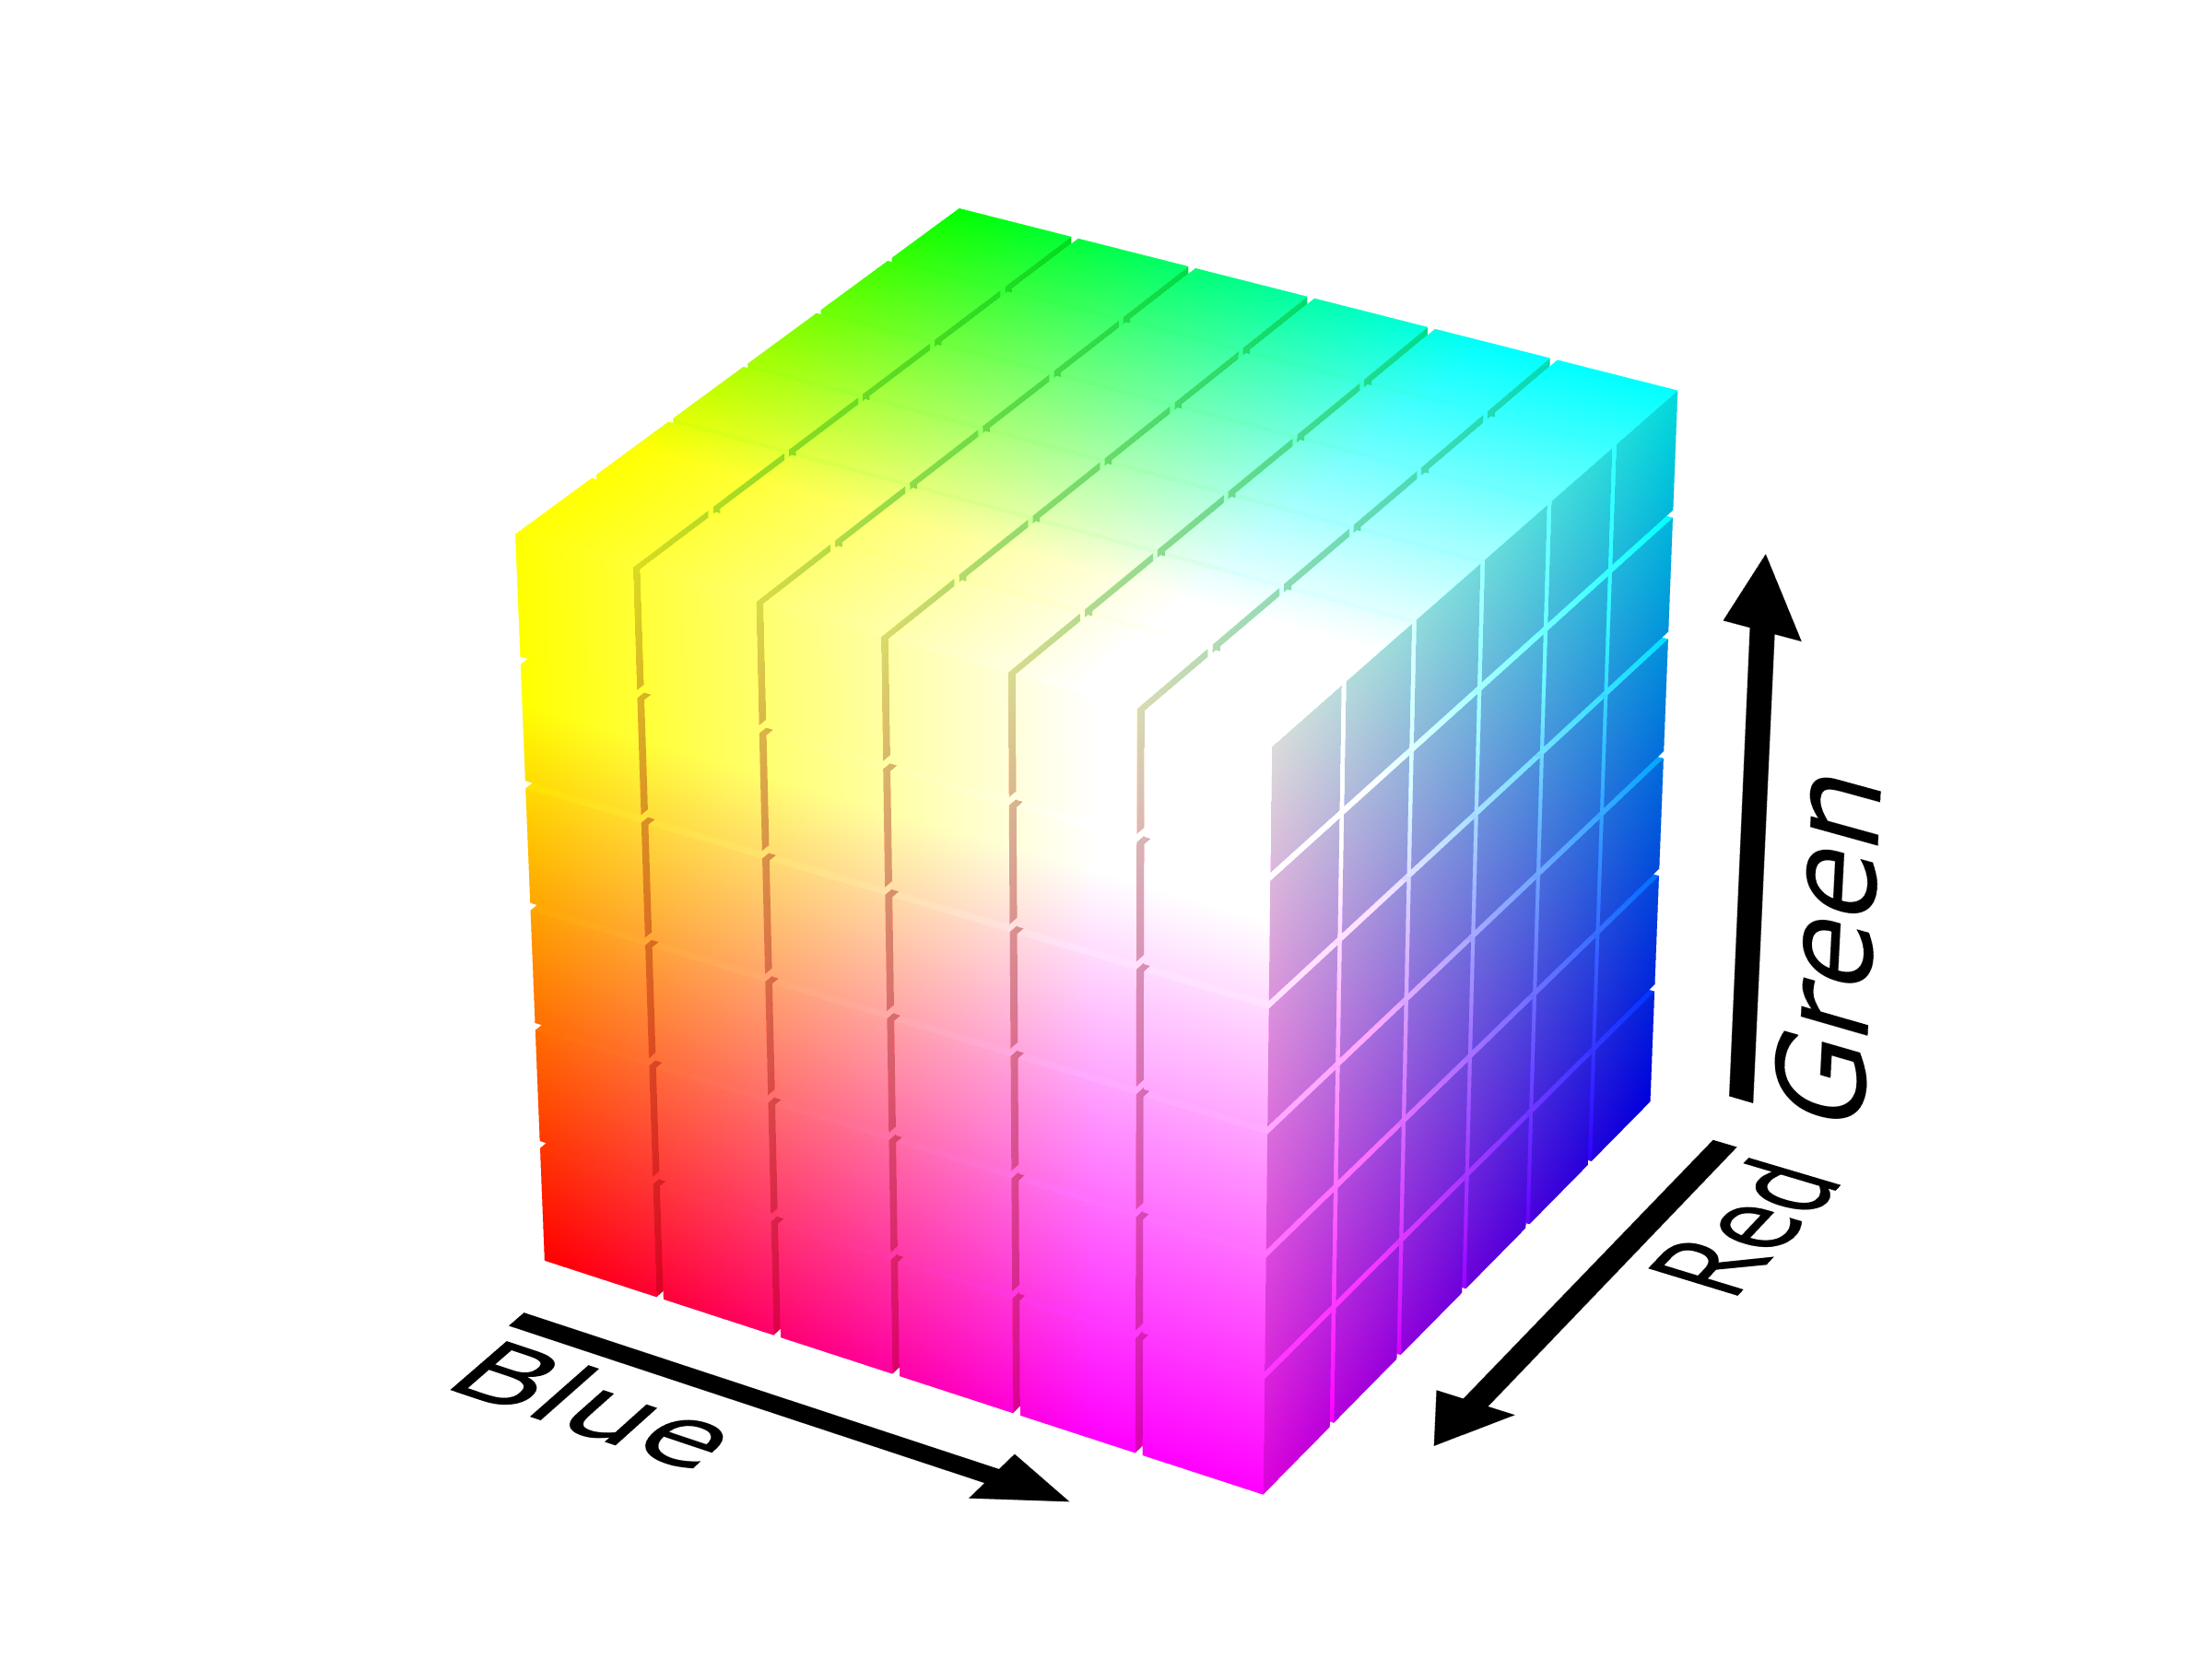
\includegraphics[width=0.4\textwidth]{img/img1.png}
	\caption{Lorem ipsum dolor sit amet}
	\label{fig:spire05}
\end{figure}


\begin{equation}
S_{p0}=\frac{T_{0} }{T_{p}} \\
\label{F:100}
\end{equation}
\begin{equation}
S_{p}=\frac{T_{1} }{T_{p}}
\label{F:101}
\end{equation}
где $T_{0}$ -- Lorem ipsum dolor sit amet, $T_{1}$ -- Lorem ipsum dolor sit amet, $T_{p}$ -- Lorem ipsum dolor sit ametLorem ipsum dolor sit amet \cite{book2}. 

Lorem ipsum dolor sit amet
\begin{equation}
1\leq S_{p} \leq p,\; \;  \frac{1}{p} \leq E_{p} \leq 1
\label{F:103}
\end{equation}



\begin{table}[h!]
	\caption{\label{tab:tbl1}Формат записи трассы PICL}
	\begin{tabular}{|l|l|}
		%	&\makebox[3em]{6/3}&\makebox[3em]{6/4}
		\hline
		Наименование поля & Назначение \\
		\hline\hline
		тип записи&тип информации в записи
		\\\hline
		тип события &тип события, с которым связана запись
		\\\hline
		отметка времени&когда информация была истинной\\\hline
		идентификатор процессора
		&процессор, с которым связана информация
		\\\hline
		идентификатор процесса	
		&процесс, с которым связана информация	
		\\\hline
		количество полей данных	
		&количество дополнительных полей данных, связанных \tabularnewline & с данными типами записи и события	
		\\\hline
		дескриптор данных	
		&формат полей данных
		\\\hline
		данные	
		&дополнительные поля данных
		\\\hline
		
	\end{tabular}
\end{table}

%%% Local Variables:
%%% mode: latex
%%% TeX-master: "rpz"
%%% End:
